\documentclass[12pt, letterpaper]{article}
\usepackage[utf8]{inputenc}
\usepackage{graphicx}
\graphicspath{ {./images/} }

\title{First document}
\author{Hubert Farnsworth \thanks{funded by the Overleaf team}}
\date{February 2014}

\begin{document}
\tableofcontents
\newpage


\section{Important Concepts in VLSI Design}

\textbf{The Complete VLSI Design Flow:}

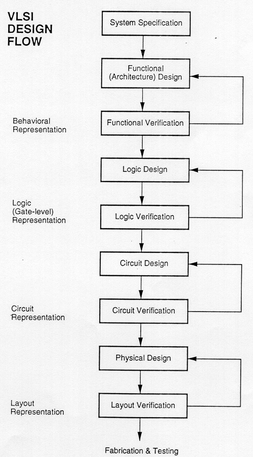
\includegraphics [scale=1.6]{vsdflow}

The VLSI Design Flow is divided into two categories:
\begin{itemize}
    \item Frontend VLSI Design
    \item Backend VLSI Design (VLSI Physical Design)
\end{itemize}

\emph{Steps in VLSI Physical Design}
\begin{itemize}
    \item Floorplanning.
    \item Partitioning.
    \item Preplaced Cells.
    \item Power Planning. (Grid Power Structure).
    \item PNR (Placement and Routing).
    \item STA (Static Timing Analysis).
\end{itemize}

The MOS Capacitance Model

Critical Path : In any digital logic circuit, the path with the maximum delay is called is called the Critical Path.

									Logical Effort
1. Introduction.
2. Basics of logical effort.
3. Calculation of logical effort for logic gates.
4. Multistage Logic Network
5. Recapitulation. 




\section{The MOS Inverter}
\subsection{The Depletion-Load nMOS Inverter}
\subsubsection{Static Characteristics}
\subsubsection{Noise Margin}
\subsubsection{Static Power Dissipation}

\subsection{The Static CMOS Inverter}
\subsubsection{Static Characteristics}
\subsubsection{Noise Margin}
\subsubsection{Static Power Dissipation}
\subsubsection{Dynamic Power Dissipation}

\section{Combinational Logic Design using MOS Transistor}

\subsection{MOS Technologies}
\begin{itemize}
    \item Depletion-Load nMOS Logic
    \item Static CMOS Logic
    \item Pseudo nMOS Logic
    \item Dynamic MOS circuits
    \begin{itemize}
        \item Single Phase Dynamic Circuits.
        \item Two Phase Dynamic Circuits. (Requires a 2 Phase Clock)
    \end{itemize}
    \item Dynamic CMOS Logic.
    \item Domino CMOS Logic.
    \item Pass Transistor Logic.
\end{itemize}

\subsection{Comparison of MOS Logic Technologies}

\subsubsection{Depletion Load nMOS Logic}
Advantages:
\begin{itemize}
    \item Requires less transistors and hence less Si area. (requires n+1 nMOS transistors for a logic circuit with fan – in ‘n’)
\end{itemize}

Disadvantages:
\begin{itemize}
    \item Limited output voltage swing.
    \item Quite high static power dissipation.
\end{itemize}

\subsubsection{Static CMOS Logic}

Advantages:
\begin{itemize}
    \item Negligible static power dissipation.
    \item Full output voltage swing.
    \item They have twice the available current drive due to both nMOS and pMOS networks.
\end{itemize}


Disadvantages:
\begin{itemize}
    \item Dynamic power disspation is proportional to operating frequency. ($CV_{DD}^2 f$)
    \item Requires a large number of transistors. (for a circuit with fan-in ‘n’ we require 2*n transistors.). This is because logic function is implemented twice.
    \item Requires greater Si area.
    \item Subsequent stage capacitances are higher due to both nMOS and pMOS networks.
    \item Longer delays due to higher load capacitances.
\end{itemize}

The basic structure of CMOS Logic:

\subsubsection{Pseudo NMOS Logic}

Advantages
\begin{itemize}
    \item Smaller area is required.
    \item Have faster rate of operation.
\end{itemize}

Disadvantages
\begin{itemize}
    \item They draw static current as long as power remains 'ON'.
    \item They used ratioed logic, so the low level logic is not strong.
\end{itemize}

\subsubsection{Dynamic MOS Logic Circuits}
The need for the smaller area of Pseudo nMOS circuits and the Power Efficiency of CMOS circuits led to the rise of \textbf{Dynamic MOS circuits}. In this circuits we exploit the inherent parasitic capacitances of MOS circuits to our benefit.

Advantages
\begin{itemize}
    \item 
\end{itemize}

Two Phase dynamic MOS circuits:


 








							Pass Transistor Logic


Transmission Gates.


The equivalent resistance of pass transistors:





\section{Concept of Memory Design}

\subsection{Outline}
\begin{itemize}
    \item Introduction to Memory.
    \item Memory Classification.
    \item Memory Architectures and Building Blocks
    \item The Memory Core.
    \item	Read-only Memories.
    \item	Non-Volatile Read-Write Memories.
    \item Read-Write Memories.
    \item Recapitulation
\end{itemize}

The Memory Core is implemented as an arrayed architecture as it helps to increase the component density of the memory chips, so as to pack larger volumes of memory in smaller areas. 
\subsection{Memory Classification}
\emph{Semiconductor Memories are broadly classified as follows:}
\begin{itemize}
    \item  Volatile Read/Write Memory.(Ex - RAM)
    \item Non-Volatile Read/Write Memory. (Ex - EROM \& EEPROM)
    \item Read-Only Memory (Masked Read-Only Memory)
\end{itemize}

Sense Amplifiers are an important component of Semiconductor Memories.

\subsubsection{RAM (Random Access Memory)}
Random Access Memories are named so because we can randomly select any particular memory cell from the memory core using the Row and Column Decoders.
Since, the memory core is densely packed with memory cells, each transistor of the memory cells are very small and hence can handle very low currents, but the \textit{data} and \textit{data bar} lines are large capacitive loads and therefore these small transistors would take a long time to charge and discharge these data lines. So, to mitigate this we use sense amplifiers to handle the switching of the states of the data lines.

\emph{RAM is classified into following two categories:}
\begin{itemize}
    \item Static RAM (SRAM)
    \item Dynamic RAM (DRAM)
\end{itemize}

\emph{The 6T SRAM Cell} \\
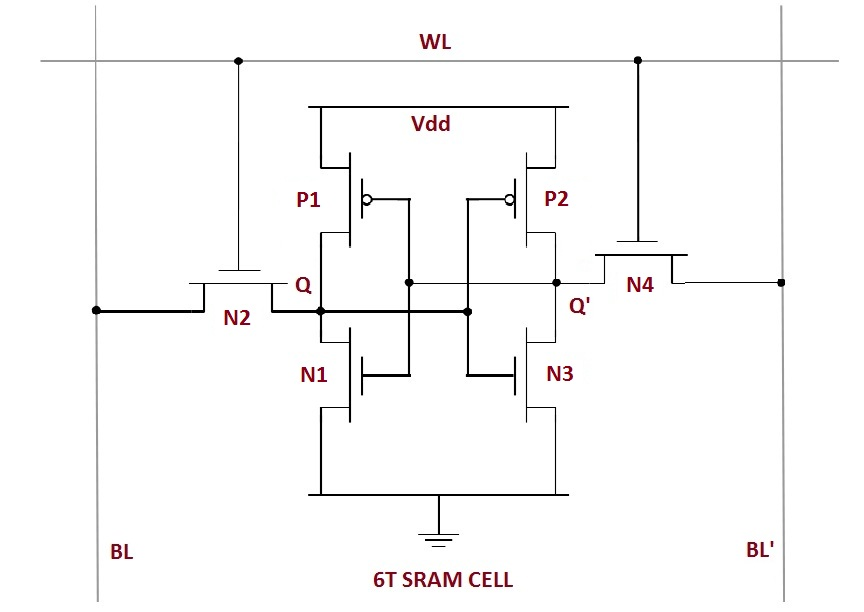
\includegraphics [scale=0.5]{sram-cell}

The block diagram of the Memory Architecture: \\
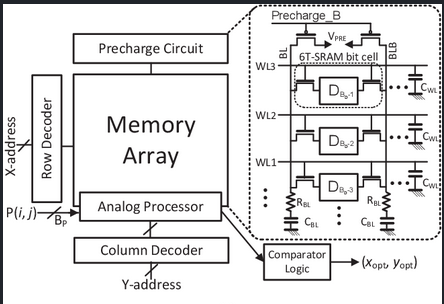
\includegraphics[scale=0.7]{det_mem_arch}

 


\end{document}







